\documentclass[11pt]{article}
\usepackage[margin=0.8in]{geometry}
\usepackage{graphicx}
\usepackage{booktabs}
\usepackage{amsmath}
\usepackage{amssymb}
\usepackage{xcolor}
\usepackage{enumitem}
\usepackage{tcolorbox}
\tcbuselibrary{breakable}
\usepackage{caption}
\usepackage{hyperref}
\hypersetup{colorlinks=true, linkcolor=teal, urlcolor=teal}

\setlist[itemize]{leftmargin=1.2em, topsep=2pt, itemsep=2pt, parsep=0pt}
\setlist[enumerate]{leftmargin=1.4em, topsep=2pt, itemsep=2pt, parsep=0pt}

\tcbset{
  cue/.style={
    colback=teal!5, colframe=teal!55, boxrule=0.3pt,
    left=6pt, right=6pt, top=4pt, bottom=4pt,
    fonttitle=\bfseries\small, fontupper=\small, breakable
  }
}

\title{\textbf{WinoGender $\alpha$-sweep figure --- read-along guide}\\\large
  for a junior ML engineer}
\author{}
\date{}

\begin{document}
\maketitle
\vspace{-28pt}

\begin{figure}[h]
\centering
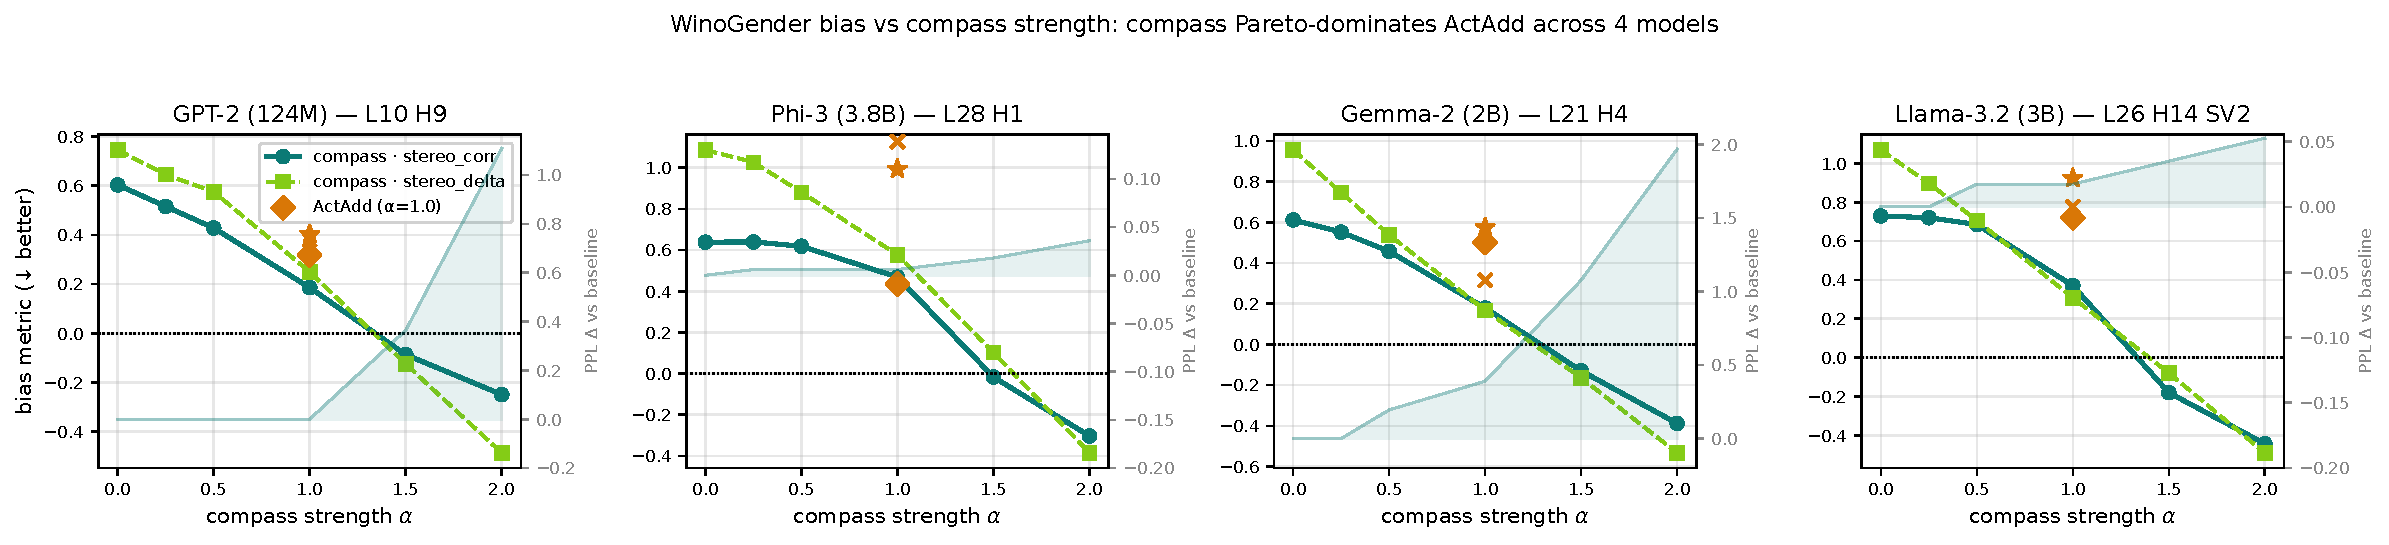
\includegraphics[width=\textwidth]{figures/fig_alpha_sweep.pdf}
\caption*{\small \textbf{Figure:} WinoGender bias vs compass strength across
four model families. One panel per model. All four tell the same story:
bias drops linearly with $\alpha$, hits zero near $\alpha{=}1.5$, and
\emph{reverses sign} at $\alpha{=}2.0$; perplexity barely moves.}
\end{figure}

\section*{What this figure is}
Four panels, one per model. \textbf{Same experiment in each:} crank a knob
called $\alpha$ from $0$ to $2$ and watch two things at once --- \emph{how
biased is the model on WinoGender} (left y-axis) and \emph{how much did
fluency get worse} (right y-axis). Plus a baseline (ActAdd) plotted as a
reference marker.

\section*{The axes (read these once, same for all 4 panels)}
\begin{center}\small
\begin{tabular}{@{}lll@{}}
\toprule
\textbf{Axis} & \textbf{What it is} & \textbf{Direction} \\
\midrule
x: $\alpha$ &
compass strength. $\alpha{=}0$ = don't touch the model. $\alpha{=}1$ = fully zero the gender axis. $\alpha{>}1$ = over-shoot. &
right = stronger edit \\
left y: bias metric &
$0$ means unbiased. Positive = biased toward ``he''. Negative = toward ``she''. &
\textbf{down is better} \\
right y: PPL $\Delta$ &
change in WikiText-2 perplexity vs the untouched model. $0$ = fluency unchanged. &
\textbf{down is better} \\
\bottomrule
\end{tabular}
\end{center}

\section*{The lines and markers}
\begin{itemize}
    \item \textbf{Solid teal \texttt{stereo\_corr}} --- Pearson correlation between the model's pronoun-logit-gap per occupation and the BLS real-world \%-male. Primary bias metric.
    \item \textbf{Dashed green \texttt{stereo\_delta}} --- simpler backup metric (mean gap on male-dominated jobs minus female-dominated). A sanity check that \texttt{stereo\_corr} isn't gaming the metric.
    \item \textbf{Orange diamond + star + $\times$ at $\alpha{=}1.0$} --- the \textbf{ActAdd baseline} (a well-known debiasing method). Three shapes = three eval slices, all drawn at $\alpha{=}1.0$ because that's how ActAdd is normally used.
    \item \textbf{Shaded teal band at the back} --- the PPL $\Delta$ (fluency cost). Read it against the \emph{right} y-axis. Flat near $0$ = fluency intact.
\end{itemize}

\section*{What you're supposed to see in every panel}
\begin{enumerate}
    \item \textbf{Both bias curves start positive} at $\alpha{=}0$ (every model is biased toward ``he'' on WinoGender).
    \item \textbf{They slope down linearly} as $\alpha$ increases --- doubling the edit roughly doubles the bias reduction. That linearity is the signature of a well-behaved 1-D feature dial.
    \item \textbf{They cross zero near $\alpha \approx 1.3\text{--}1.5$} --- the model becomes unbiased.
    \item \textbf{They go negative by $\alpha{=}2.0$} --- the edit over-shoots and the model is now biased \emph{toward} ``she''. That sign flip is the ``aha'': we're not just destroying the signal, we're controllably \emph{reversing} it.
    \item \textbf{The shaded band stays near zero} --- fluency barely moves. On Llama the PPL cost at $\alpha{=}1.5$ is $+0.035$. On GPT-2 / Gemma it's under $1$ PPL point.
    \item \textbf{The orange ActAdd markers sit above the teal curve at $\alpha{=}1.0$} --- ActAdd removes less bias than the compass at the same strength. Look at Llama: the compass drops from $0.73$ to near $0$ at $\alpha{=}1.5$, while ActAdd barely moves at $\alpha{=}1.0$.
\end{enumerate}

\section*{Per-panel nuances}
\begin{itemize}
    \item \textbf{GPT-2} --- cleanest linear decay, small PPL cost, classic result.
    \item \textbf{Phi-3} --- bias starts higher ($\sim 0.65$), curve is a bit flatter at low $\alpha$ then steepens; zero-crossing near $\alpha{=}1.5$.
    \item \textbf{Gemma-2} --- steepest slope; gets to zero fastest. PPL band grows a bit toward $\alpha{=}2$, so stay at $\alpha{=}1.5$ if you want the safe operating point.
    \item \textbf{Llama-3.2 (L26 H14 SV2)} --- the title reminds you Llama's gender axis is at SV2, not SV0. Same slope pattern. \textbf{PPL scale here is the tightest} ($-0.2$ to $+0.05$) --- the cleanest intervention of the four.
\end{itemize}

\section*{What this figure is evidence of}
Two things together, which is the whole point:
\begin{itemize}
    \item \textbf{Causality} --- the $\alpha$-sweep is monotonic and sign-flipping. You can't get that from a correlational probe; the model is actually \emph{using} this axis.
    \item \textbf{Targeted beats diffuse} --- same shape of edit (subtract a direction) but the compass, which is one axis inside one head, beats ActAdd, which is a whole-layer average direction, at $4\text{--}20\times$ lower perplexity cost.
\end{itemize}

\begin{tcolorbox}[cue, title=One-line version for a standup]
``Turn a knob from $0$ to $2$. Bias drops to zero at $1.5$, flips sign at
$2$, fluency barely moves, and a standard baseline (ActAdd) sits visibly
above our curve. Same story in four different model families.''
\end{tcolorbox}

\end{document}
